145. \begin{figure}[ht!]
\center{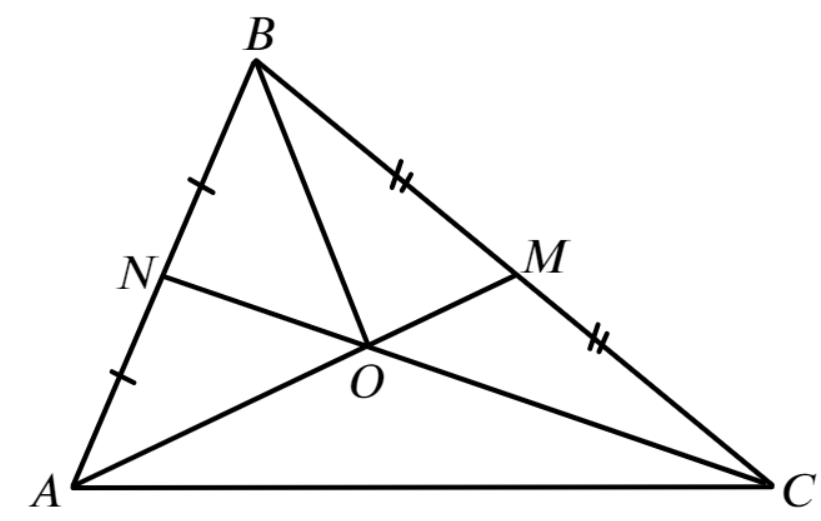
\includegraphics[scale=0.35]{g9-145.png}}
\end{figure}\\
Так как площади треугольников, имеющих общую высоту, относятся как стороны, к которым она проведена, обозначим $S_c{\Delta ANO}=S_{\Delta BNO}=x,\ S_{\Delta BMO}=S_{\Delta CMO}=y.$ Так как $CO:ON=2:1,$ получим $2y:x=2:1,$ то есть $x=y.$ Также $S_{\Delta AOC}:S_{\Delta AON}=2:1,$ значит $S_{\Delta AOC}=2x.$ Таким образом, $\cfrac{S_{NBMO}}{S_{\Delta ABC}}=\cfrac{2x}{6x}=\cfrac{1}{3}.$\\
